\documentclass[a4paper,12pt,oneside,openany]{book}	

\usepackage{layout}
\usepackage[english,brazil]{babel}
\setlength{\textheight}{25.0 cm}


\usepackage{indentfirst}		% for indent

\usepackage[T1]{fontenc} 
\usepackage[utf8]{inputenc}
\usepackage[hidelinks]{hyperref}


\usepackage{epsfig}
\usepackage{float}
\usepackage{graphicx}
\usepackage[justification=centering]{caption}
\usepackage{subcaption}


\usepackage{tabularx}

\graphicspath{{./images/}}
\usepackage{pstricks,pst-node,pst-tree}
\usepackage{alltt}
%\usepackage{makeidx}
%\makeindex
\usepackage[figuresright]{rotating} % for saydways tables and figures
\usepackage{enumerate}			% for configuration of enumerate environment
\usepackage{amsmath}
\usepackage{amssymb}
\usepackage{portland,multirow}

\setcounter{secnumdepth}{3}	% numeracao ate subsubsecao
\setcounter{tocdepth}{2}	% indice ate subsubsecao

\usepackage{longtable}




\begin{document}
	

\frontmatter

\thispagestyle{empty}



\begin{center}
\large{ESTUDO E DESENVOLVIMENTO DE ALGORITMOS DE CONTROLE ADAPTATIVOS PARA ELETROESTIMULAÇÃO NEUROMUSCULAR VOLTADA PARA FISIOTERAPIA}\\
   \vspace{2cm}
\large{Luiz Rennó Costa}\\
\end{center}
   \vspace{3cm}
\hspace{7cm}
\hfill \parbox{8.0cm}{Projeto de Graduação apresentado ao Curso de Engenharia Eletrônica e de Computação da Escola Politécnica, Universidade Federal do Rio de Janeiro, como parte dos requisitos necessários à obtenção do título de Engenheiro.\\}
   \vspace{2cm}
\hfill \parbox{8.0cm}{Orientadores: Alexandre Visintainer Pino \\ Tiago Roux de Oliveira} \\
   \vspace{2cm}
\begin{center}
Rio de Janeiro

Outubro de 2008
\end{center}




\pagebreak


\begin{center}
\large{ESTUDO E DESENVOLVIMENTO DE ALGORITMOS DE CONTROLE ADAPTATIVOS PARA ELETROESTIMULAÇÃO NEUROMUSCULAR VOLTADA PARA FISIOTERAPIA}\\
   \vspace{1cm}
\large{Luiz Rennó Costa}\\
\end{center}
   \vspace{2cm}
PROJETO DE GRADUAÇÃO SUBMETIDO AO CORPO DOCENTE DO CURSO DE ENGENHARIA ELETRÔNICA E DE COMPUTAÇÃO DA ESCOLA POLITÉCNICA DA UNIVERSIDADE FEDERAL DO RIO DE JANEIRO COMO PARTE DOS REQUISITOS NECESSÁRIOS PARA A OBTENÇÃO DO GRAU DE ENGENHEIRO ELETRÔNICO E DE COMPUTAÇÃO   
   
   \vspace{1cm}
Autor:
      \vspace{0.5cm}
      \begin{flushright}
         \parbox{10cm}{
            \hrulefill

            \vspace{-.375cm}
            \centering{Luiz Rennó Costa}

            \vspace{0.1cm}
         }
      \end{flushright}
      
      
Orientadores:
      \vspace{0.5cm}
      \begin{flushright}
         \parbox{10cm}{
            \hrulefill

            \vspace{-.375cm}
            \centering{Prof. Alexandre Visintainer Pino, Ph. D.}
            \centering{Prof. Tiago Roux de Oliveira, Ph. D.}

            \vspace{0.1cm}
         }
      \end{flushright}
      
Examinador:
      \vspace{0.5cm}
      \begin{flushright}
         \parbox{10cm}{
            \hrulefill

            \vspace{-.375cm}
            \centering{Prof Frances Elizabeth Allen, D. Sc.}

            \vspace{0.1cm}
         }
      \end{flushright}
      
Examinador:
      \vspace{0.5cm}
      \begin{flushright}
         \parbox{10cm}{
            \hrulefill

            \vspace{-.375cm}
            \centering{Prof. Alan Jay Perlis, D. E.}

            \vspace{0.1cm}
         }
      \end{flushright}
      
                        
      \vfill
      
      
\begin{center}
Rio de Janeiro

Outubro de 2008
\end{center}


%\pagebreak            

\begin{center}
	Declaração de Autoria e de Direitos
\end{center}

\vspace{0.5cm}

Eu, \emph{Luiz Rennó Costa} CPF \emph{135.601.997-86}, autor da monografia \emph{ESTUDO E DESENVOLVIMENTO DE ALGORITMOS DE CONTROLE ADAPTATIVOS PARA ELETROESTIMULAÇÃO NEUROMUSCULAR VOLTADA PARA FISIOTERAPIA}, subscrevo para os devidos fins, as seguintes informações:\\
1. O autor declara que o trabalho apresentado na disciplina de Projeto de Graduação da Escola Politécnica da UFRJ é de sua autoria, sendo original em forma e conteúdo.\\
2. Excetuam-se do item 1. eventuais transcrições de texto, figuras, tabelas, conceitos e idéias, que identifiquem claramente a fonte original, explicitando as autorizações obtidas dos respectivos proprietários, quando necessárias.\\
3. O autor permite que a UFRJ, por um prazo indeterminado, efetue em qualquer mídia de divulgação, a publicação do trabalho acadêmico em sua totalidade, ou em parte. Essa autorização não envolve ônus de qualquer natureza à UFRJ, ou aos seus representantes.\\
4. O autor pode, excepcionalmente, encaminhar à Comissão de Projeto de Graduação, a não divulgação do material, por um prazo máximo de 01 (um) ano, improrrogável, a contar da data de defesa, desde que o pedido seja justificado, e solicitado antecipadamente, por escrito, à Congregação da Escola Politécnica.\\
5. O autor declara, ainda, ter a capacidade jurídica para a prática do presente ato, assim como ter conhecimento do teor da presente Declaração, estando ciente das sanções e punições legais, no que tange a cópia parcial, ou total, de obra intelectual, o que se configura como violação do direito autoral previsto no Código Penal Brasileiro no art.184 e art.299, bem como na Lei 9.610.\\
6. O autor é o único responsável pelo conteúdo apresentado nos trabalhos acadêmicos publicados, não cabendo à UFRJ, aos seus representantes,  ou ao(s) orientador(es), qualquer responsabilização/ indenização nesse sentido.\\
7. Por ser verdade, firmo a presente declaração.\\

\vspace{0.5cm}
\begin{flushright}
	\parbox{10cm}{
		\hrulefill
		
		\vspace{-.375cm}
		\centering{Luiz Rennó Costa}
		
		\vspace{0.1cm}
	}
\end{flushright}

\pagebreak

% Copyright
\vspace{0.5cm}

UNIVERSIDADE FEDERAL DO RIO DE JANEIRO \\
Escola Politécnica - Departamento de Eletrônica e de Computação \\
Centro de Tecnologia, bloco H, sala H-217, Cidade Universitária \\ 
Rio de Janeiro - RJ      CEP 21949-900\\
\vspace{0.5cm}
\paragraph{}Este exemplar é de propriedade da Universidade Federal do Rio de Janeiro, que poderá incluí-lo em base de dados, armazenar em computador, microfilmar ou adotar qualquer forma de arquivamento.
\paragraph{}É permitida a menção, reprodução parcial ou integral e a transmissão entre bibliotecas deste trabalho, sem modificação de seu texto, em qualquer meio que esteja ou venha a ser fixado, para pesquisa acadêmica, comentários e citações, desde que sem finalidade comercial e que seja feita a referência bibliográfica completa.
\paragraph{}Os conceitos expressos neste trabalho são de responsabilidade do(s) autor(es).

%
\pagebreak
%%%
% Dedicatória
\begin{center}
	\textbf{DEDICATÓRIA}
\end{center}
\vspace{0.5cm}

\paragraph{}Opcional.

\pagebreak


% Agradecimento
\begin{center}
	\textbf{AGRADECIMENTO}
\end{center}
\vspace{0.5cm}

\paragraph{}Sempre haverá. Se não estiver inspirado, aqui está uma sugestão: dedico este trabalho ao povo brasileiro que contribuiu de forma significativa à minha formação e estada nesta Universidade. Este projeto é uma pequena forma de retribuir o investimento e confiança em mim depositados.

\pagebreak


% Resumo
\begin{center}
	\textbf{RESUMO}
\end{center}
\vspace{0.5cm}

\paragraph{}Para o tratamento de pessoas acometidas de sequelas físicas provindas de AVC, é necessário passar por diversas sessões de fisioterapia. Para aumentar a eficiência deste tratamento, dispositivos auxiliares de eletroestimulação foram desenvolvidos. Este trabalho tenta maximizar a eficiência do tratamento por meios de desenvolvimento de técnicas de controle suficientemente robustas, para tornar o aparelho o mais autônomo possível.
\paragraph{}
\noindent Palavras-Chave: eletroestimulação, NMES, AVC, tratamento, fisioterapia, eletroterapia

\pagebreak


% Abstract
\begin{center}
	\textbf{ABSTRACT}
\end{center}
\vspace{0.5cm}

\paragraph{}Insert your abstract here. Insert your abstract here. Insert your abstract here. Insert your abstract here. Insert your abstract here.
\paragraph{}
\noindent Key-words: word, word, word.

\pagebreak


% Siglas
\begin{center}
	\textbf{SIGLAS}
\end{center}
\vspace{0.5cm}

\paragraph{}UFRJ - Universidade Federal do Rio de Janeiro 
\paragraph{}NMES - \textit{Neuromuscular Electrical Stimulation}
\paragraph{}AVC - Acidente Vascular Cerebral
\paragraph{}OMS - Organização Mundial da Saúde
\paragraph{}WHO - \textit{World Health Organization}

\pagebreak

% Table of Contents
% ---------------------------------------------------------------
\tableofcontents
% ---------------------------------------------------------------
% Lista de figuras
% ---------------------------------------------------------------
%\cleardoublepage
%\addcontentsline{toc}{chapter}{Lista de Figuras}
\listoffigures
% ---------------------------------------------------------------
% Lista de Tabelas
% ---------------------------------------------------------------
%\cleardoublepage
%\addcontentsline{toc}{chapter}{Lista de Tabelas}
\listoftables

\mainmatter
\cleardoublepage
% ---------------------------------------------------------------
% Chapter 1 - Introdução
% ---------------------------------------------------------------
\chapter{Introdução}
\label{intro_cap1}
\section{Tema}

\paragraph{}Pessoas acometidas por acidente vascular cerebral (AVC) desenvolvem sequelas cognitivas (impedimento de fala, problemas de concentração) e físicas (espasticidade, paralisia parcial). O trabalho focará em apenas uma sequela física, a espasticidade.

\paragraph{}Para o tratamento da espasticidade, o paciente deve passar por sessões de fisioterapia, aonde realizará movimentos com a ajuda do médico. Com o avanço da tecnologia, novas formas de tratamento surgiram, se baseando principalmente na eletroestimulação neuromuscular (NMES).

\paragraph{}Para a realização de tal tratamento de maneira eficiente, é necessário um dispositivo auxiliar que seja capaz de se adaptar aos diferentes tipos de pacientes com variados níveis e tipos de lesões.

\paragraph{}Este trabalho então, estuda e avalia a eficácia de diferentes algoritmos de controle para o tratamento de espasticidade provinda do AVC através de eletroestimulação neuromuscular.


\section{Delimitação}

\paragraph{}------------------------------------------------------


\section{Justificativa}

\paragraph{}Tais dispositivos auxiliares discutidos anteriormente são escassos e caros no Brasil (existem apenas alguns importados) e destes, nenhum possui a realimentação do paciente, ele é operado em malha aberta, o que requer um conhecimento específico do médico (diminuindo a capacidade de atuação do aparelho) e diminui a eficácia do tratamento. Portanto o desenvolvimento deste dispositivo poderia ajudar na recuperação de milhares de pacientes da maneira mais eficaz possível.

\section{Objetivos}

\paragraph{}O objetivo deste trabalho é estudar e desenvolver técnicas de controle robustas e suficiente adaptativas para utilização com NMES voltada para fisioterapia no tratamento de espasticidade. No futuro, com a realização e implementação bem sucedida deste, se espera um aparelho autônomo, que não precise de calibração por parte do médico, e se adapte à toda (ou quase toda) situação clínica no tratamento da espasticidade.


\section{Metodologia}

\paragraph{}Como é a abordagem do assunto. Como foi feita a pesquisa, se vai houve validação, etc. Em resumo, você de explicar qual foi sua estratégia para atender ao objetivo do trabalho (tamanho do texto: livre).


\section{Descrição}

\paragraph{}No capítulo 2 será feito uma revisão de todo o conteúdo necessário para o entendimento do trabalho, especialmente dos termos médicos e técnicos que serão usados posteriormente.

\paragraph{}O capítulo 3 apresenta ...

\paragraph{}Os .... são apresentados no capítulo 4. Nele será explicitado ...

\paragraph{}E assim vai até chegar na conclusão.


% ---------------------------------------------------------------
% Chapter 2 - Background Info
% ---------------------------------------------------------------
\chapter{Background}
	\label{background_cap2}
	\section{Biomédica}

	\paragraph{} Nesta sessão todo o conhecimento necessário sobre a parte de biomédica será apresentado, para garantir o entendimento do leitor.
	
	\subsection{Acidente Vascular Cerebral}
	
	\paragraph{}A definição utilizada pela Organização Mundial da Saúde, OMS (ou \textit{World Health Organization}, WHO) é "desenvolvimento rápido de sinais clínicos de distúrbios regionais (ou globais) da função cerebral, durando mais do que 24 horas ou resultando em morte, com nenhuma outra causa aparente além de ter sido de origem vascular."\cite{Cerebrov82} Atualmente novas definições vem sendo estudadas para se tornarem mais compatíveis com o avanço da tecnologia.\cite{Sacco2064}
	
	\paragraph{}Existem dois tipos de AVC, isquêmico e hemorrágico, o primeiro é o tipo mais usual, e consiste em um impedimento de fornecimento de sangue para o cérebro por meio de um coágulo sanguíneo. O último é o tipo mais letal, e ocorre por meio de uma hemorragia, causando inchaço e pressão no cérebro, tais acontecimentos causam morte dos neurônios e do tecido cerebral.
	
	\begin{figure}[H]
		\centering
		\begin{subfigure}{0.5\textwidth}
			\centering
			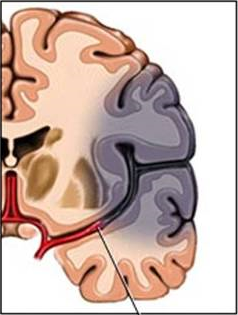
\includegraphics[width=0.5\textwidth]{isc_avc}
			\caption{AVC isquêmico}
			\label{fig:isq_avc}
		\end{subfigure}~
	\begin{subfigure}{0.5\textwidth}
			\centering
			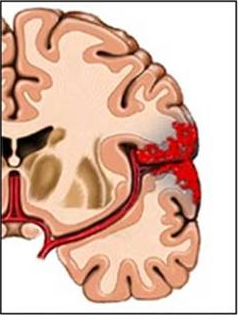
\includegraphics[width=0.5\textwidth]{hemo_avc}
			\caption{AVC hemorrágico}
			\label{fig:hemo_avc}
		\end{subfigure}
		\caption{Comparação entre os dois tipos de AVC}
	\end{figure}


	\subsection{Espasticidade}
	\paragraph{}"A espasticidade é uma desordem motora caracterizada por um aumento do tônus muscular [...] resultando da hiperexcitabilidade do reflexo de extensão".\cite{Lance80} Tônus muscular é a contração contínua e passiva do músculo, ou seja, o quão contraído o membro está quando em repouso.
	
	\begin{figure}[H]
		\centering
		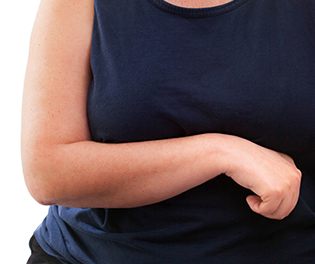
\includegraphics[width=0.5\textwidth]{spas_ex}
		\caption{Paciente com espasticidade}
		\label{fig:spasticity}
	\end{figure}
	
	\paragraph{}Este trabalho focará mais em espasticidade dos membros superiores (bíceps e tríceps). Para medir o grau da lesão, é utilizada a escala de Ashworth.
	
	\subsubsection{Escala de Ashworth}
	\paragraph{}A escala de Ashworth mede a resistência do movimento passivo, e é utilizada para quantificar o grau de espasticidade.
	
	\begin{table}[H]
		\centering
		\caption{Escala de Ashworth para Classificação da Espasticidade}
		\label{tab:ashworth}
	\begin{tabularx}{\textwidth}{|l X|}

		\hline
		\multicolumn{1}{|c}{Grau} & \multicolumn{1}{c|}{Descrição}                                                                                                            \\ \hline
		0                          & Nenhum aumento do tônus muscular                                                                                                          \\ \hline
		1                          & Pequeno aumento do tônus muscular, se expressando em uma minima resistência no final no movimento de extensão e flexão                    \\ \hline
		1+                         & Pequeno aumento do tônus muscular, se expressando em uma minima resistência em até metade do movimento de extensão e flexão               \\ \hline
		2                          & Médio aumento do tônus muscular, e uma resistência maior em grande parte do movimento de extensão e flexão, mas ainda move com facilidade \\ \hline
		3                          & Considerável aumento do tônus muscular, e dificuldade de realização do movimento de extensão e flexão                                     \\ \hline
		4                          & Grande aumento do tônus muscular, e as partes afetadas se tornam rígidas na extensão e flexão.\\ \hline
	\end{tabularx}
	\end{table}

\subsubsection{Escala de Rankin Modificada}

\paragraph{}A escala de Rankin\cite{Rankin57}, assim como a de Ashworth, mede a capacidade funcional do paciente acometido de AVC, a versão mais utilizada é a escala de Rankin modificada \cite{Swieten88}, que é uma escala de 6 pontos de simples classificação, indo desde falta total de sintomas, até a morte.

	\begin{table}[H]
	\centering
	\caption{Escala de Rankin Modificada}
	\label{tab:rankin}
	\begin{tabularx}{\textwidth}{|l X|}
		
		\hline
		\multicolumn{1}{|c}{Grau} & \multicolumn{1}{c|}{Descrição}                                                                                                            \\ \hline
		0                          & Nenhum sintoma e nenhuma limitação.                                                                                                          \\ \hline
		1                          & Sem deficiência motora apesar de possuir sintomas; pode executar todas as tarefas e atividades usuais.                    \\ \hline
		2                          & Deficiência leve; não pode executar todos as tarefas, mas consegue cuidar de suas necessidades básicas seu auxilio.\\ \hline
		3                          & Deficiência moderada; necessita de auxílio mas consegue andar sozinho.\\ \hline
		4                          & Deficiência forte; não consegue andar nem atender necessidades corporais sem auxílio.\\ \hline
		5                          & Deficiência severa; requer constante atenção e cuidado, acamado e incontinente. \\ \hline
	\end{tabularx}
\end{table}
	
	
	
	
	
	

% ---------------------------------------------------------------
% Chapter 3 - Metodologia
% ---------------------------------------------------------------
	\chapter{Metodologia}
	\label{Metodologia_cap3}
	\section{Instrumentação}
\paragraph{}Nesta sessão todos os instrumentos utilizados para o desenvolvimento do projeto serão descritos e a metodologia dos testes que foram realizados.

\subsection{Eletroestimulador}
\paragraph{}O eletroestimulador foi desenvolvido no Laboratório de Instrumentação Biomédica (LIB) como projeto de final de curso do aluno Anderson Francisco da Costa Souza\cite{Anderson34}, ele é constituído basicamente de um microcontrolador ALGUMACOISA que realiza a comunicação com o computador, além de providenciar o pulso de estimulação. Este pulso depois passa por diversos circuitos até passar em um estágio de saída em par Darlington para injetar a corrente no músculo.

\subsubsection{Pulso de Estimulação}

\begin{figure}[H]
	\centering
	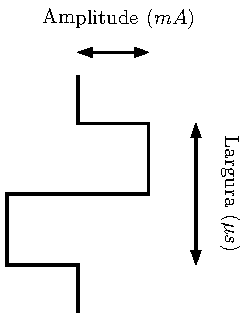
\includegraphics[width=0.5\textwidth,angle=90]{pulso_estimulacao.pdf}
	\caption{Pulso de estimulação utilizado, podendo-se variar tanto amplitude quanto largura do pulso.}
	\label{fig:pulso_estimulacao}
\end{figure}

\paragraph{}O pulso de estimulação possui formato bifásico, e é possível modificar amplitude, largura e frequência através de \textit{software}.

\subsubsection{Eletrodos de Contato}
Os eletrodos de contato utilizados foram eletrodos quadrados, autoadesivos de $5 x 5 cm$.

\subsection{Goniômetro}

\begin{figure}[H]
	\centering
	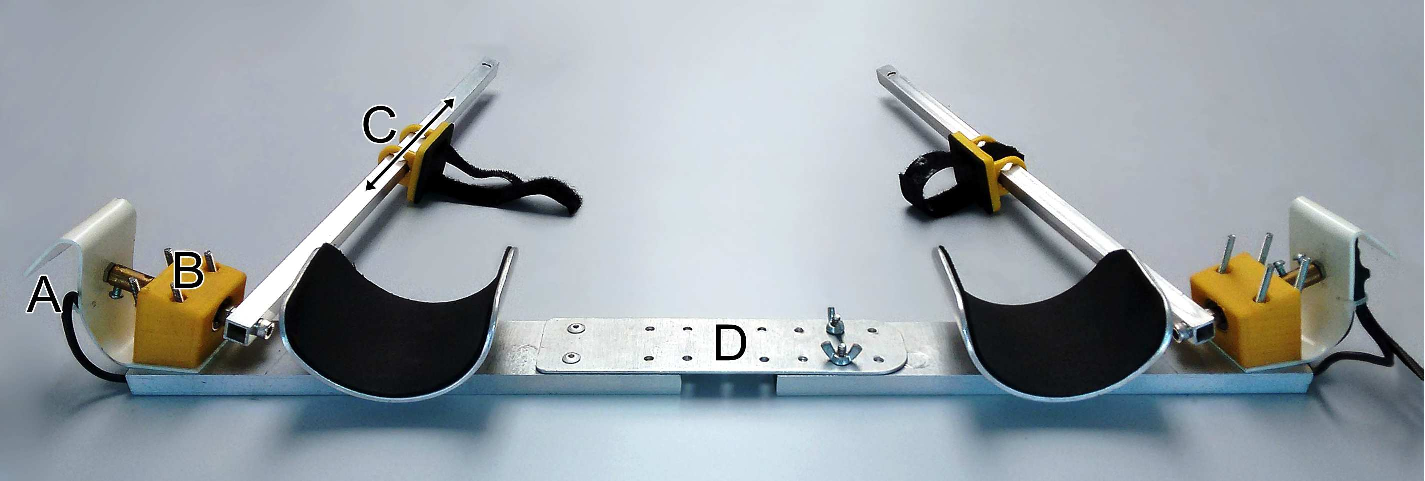
\includegraphics[width=0.8\textwidth]{aparatops.pdf}
	\caption{Goniômetro desenvolvido pelo LIB. (A) e (B) formam um conjunto de sensores, (C) é um prendedor regulável, e (D) é um regulador da largura do goniômetro.}
	\label{fig:aparatops}
\end{figure}

\subsection{Interface com o Usuário}

\begin{figure}[H]
	\centering
	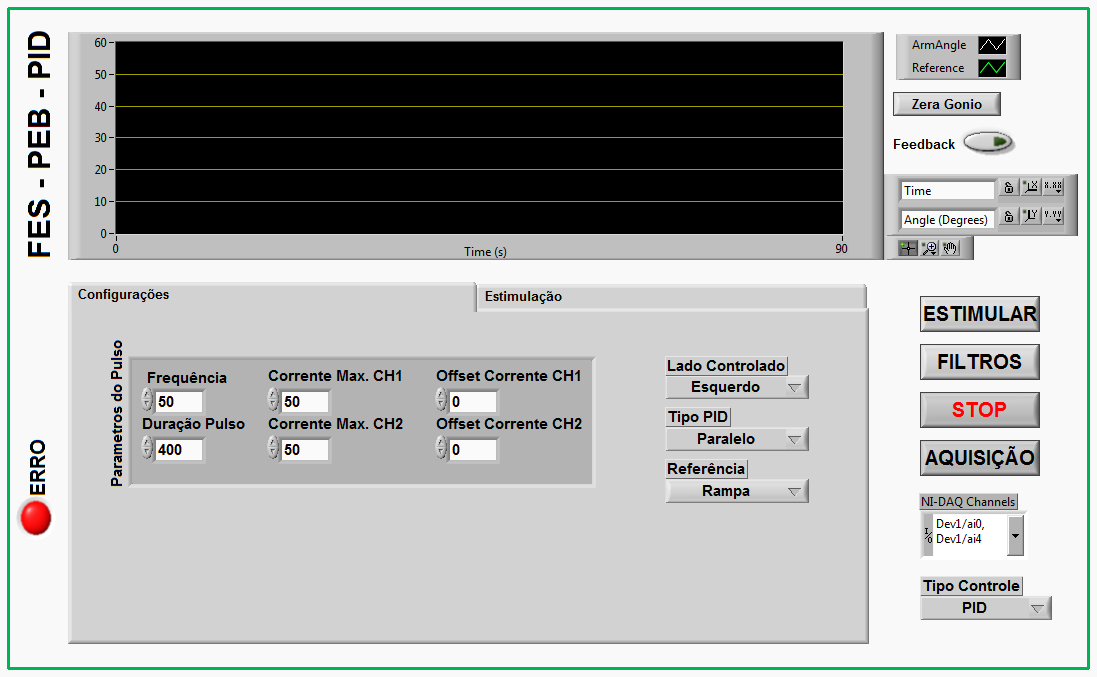
\includegraphics[width=0.8\textwidth]{interface_labview}
	\caption{Tela principal da interface de operação do \textit{software}. Feito em LabVIEW 8.5.}
	\label{fig:interface_labview}
\end{figure}

\paragraph{}A interface com o usuário, explicitada na \ref{fig:interface_labview} possui várias características importantes, um gráfico de exibição em tempo real do ângulo de referência e o do paciente, uma aba de configuração aonde são modificados os parâmetros do pulso, e qual lado está sendo controlado, além de qual estrutura do PID será utilizada, e permite a escolha da referência tanto em rampa quanto contra lateral \ref{label}.

\paragraph{}Os botões na lateral direita fazem o controle de aquisição de dados em tempo real, início da eletroestimulação, e aplicação de filtros para suavizar a referência utilizada \ref{label}. Além de dar a opção de escolher qual dispositivo de aquisição de dados usar, e qual algoritmo de controle a ser implementado.

\subsubsection{\textit{Feedback} Visual}

\begin{figure}[H]
	\centering
	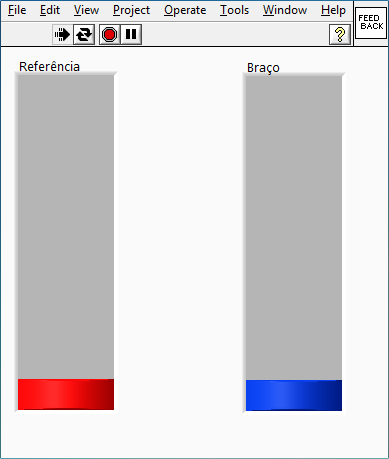
\includegraphics[width=0.8\textwidth]{feedback_visual}
	\caption{Informação visual do ângulo realizado (azul) e a referência (vermelho) em tempo real, com formato de barras crescentes.}
	\label{fig:feedback_visual}
\end{figure}

\paragraph{}O botão de \textit{Feedback} abre a janela de realimentação visual (\ref{fig:feedback_visual}) para os testes com pacientes, aonde a barra azul representa o ângulo realizado em tempo real pelo paciente, e a barra azul a referência.

\section{Testes}
\paragraph{}Para determinar a eficácia do algoritmo, testes com voluntários saudáveis e pacientes acometidos de AVC foram realizados, com isto, um protocolo de testes foi determinado e medidas estatísticas foram efetuadas com o intuito de quantizar esta eficácia.

\paragraph{}Para a realização destes, a pessoa deve ser posicionada no aparato mostrado na \ref{fig:aparatops}, e o ângulo a ser medido no teste é o ângulo $y$ em relação à mesa, exemplificado abaixo.

\begin{figure}[H]
	\centering
	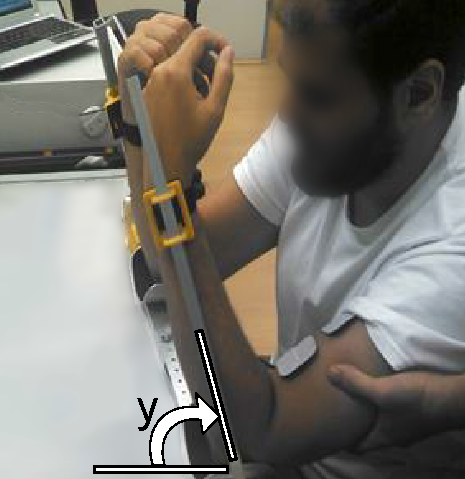
\includegraphics[width=0.6\textwidth]{fig4_new.pdf}
	\caption{Voluntário posicionado no aparelho para a realização dos testes.}
	\label{fig:thiago_anguloy}
\end{figure}


\subsection{Protocolo}
\paragraph{}O protocolo desenvolvido para os testes define o tipo de movimento que o voluntário ou paciente deverá fazer, quais músculos serão estimulados, quais parâmetros de estimulação serão usados e qual é o perfil do voluntário ou paciente passível de realizar o teste.

\paragraph{}O movimento a ser realizado consiste em uma rampa de flexão, um platô de flexão em $45\circ$, depois uma descida em rampa de extensão e finalmente um platô de extensão à $0\circ$.

\begin{figure}[H]
	\centering
	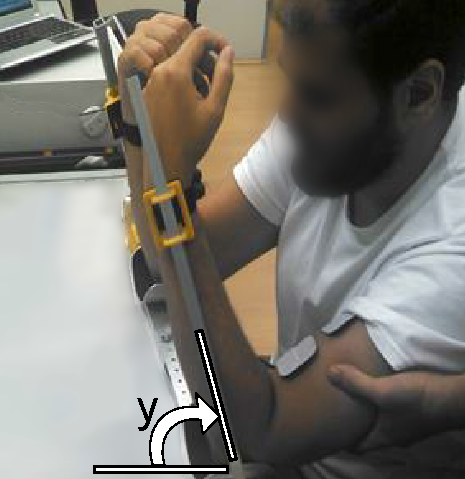
\includegraphics[width=0.5\textwidth]{fig4_new.pdf}
	\caption{Movimento a ser realizado.}
	\label{fig:protocol_mov}
\end{figure}

\paragraph{}Os músculos a serem estimulados serão exclusivamente o bíceps e o tríceps, apenas estimulação de membro superior. Isto foi determinado pois diminui razoavelmente o custo, tendo em vista que os eletrodos para estimulação de membros inferiores são bem maiores e caros.

\paragraph{}Para recrutar os voluntários e pacientes com AVC, foi feita uma triagem dos requerimentos necessários, resumidos abaixo:

\begin{itemize}
	\item Voluntários saudáveis:
	\begin{itemize}
		\item Homens e mulheres de pelo menos 20 anos
		\item 
	\end{itemize}
	\item Pacientes com AVC:
	\begin{itemize}
		\item Possuir um grau de espasticidade mínimo 0 e máximo 3 na escala de Ashworth (\ref{tab:ashworth})
		\item Ser capaz de passar no Mini Mental Test (JOAO!!!)
		\item Mínima capacidade cognitiva (JOAO!!!)
		\item Não ter aplicado BOTOX, ou aplicado à muito tempo
		\item Possuir, em estado de repouso, a capacidade de estender o braço completamente para se posicionar no goniômetro
	\end{itemize}
\end{itemize}

\paragraph{}Antes do início da coleta de dados, é necessário encontrar o ponto motor do músculo. Para fazer isto, foi determinado um procedimento que consiste em estimular o músculo utilizando um eletrodo caneta de $1 cm^{2}$ aumentando gradativamente a amplitude do pulso de estimulação com $1Hz$ de frequência e $400\mu s$ de largura, até que seja observada contração muscular. Após encontrar o ponto aonde a contração seja máxima (mantendo agora a amplitude do pulso fixa), o eletrodo deve ficar posicionado em cima deste.

\paragraph{}Após localizar o ponto motor, um procedimento para determinar a quantidade mínima e máxima de estimulação deve ser feito, este consiste em estimular (agora com os eletrodos fixos) um músculo de cada vez com amplitudes cada vez maiores, usando um pulso agora de $50Hz$ e $400\mu s$. A amplitude que gera a menor contração perceptível deve ser tomada como limite inferior, e a que causa desconforto deve ser tomada como limite superior. Desta forma, podemos realizar os testes com maior facilidade, diminuindo o efeito de zona morta do músculo e evitando desconforto do paciente.

\paragraph{}Depois de todas estas rotinas, o voluntário já poderá realizar o teste de movimento. No contexto de voluntários saudáveis, é necessário que o mesmo se mantenha o mais relaxado possível, com o intuito de não interferir na ação do controlador. Ele também não poderá ter nenhuma ajuda visual ou conhecimento prévio do movimento a ser realizado.

\paragraph{}No contexto de pacientes acometidos por AVC, é necessário que ele atue com o controlador, tendo total conhecimento do movimento a ser realizado, e a ajuda de um estímulo visual em formato de barras (\ref{fig:feedback_visual}), deverá ser instruido ao paciente que ele tente igualar o nível delas.


% ---------------------------------------------------------------
% Bibliografia
% ---------------------------------------------------------------
\normalsize
\cleardoublepage
\addcontentsline{toc}{chapter}{Bibliografia}
\bibliographystyle{coppe}
\bibliography{biblio}

% ---------------------------------------------------------------
% Apêndices 
% ---------------------------------------------------------------
\appendix
% ---------------------------------------------------------------
% Apêndice A
% ---------------------------------------------------------------
%	\chapter{O que é um apêndice}
%	\label{ApendiceA}
%	\input{ApendiceA}
% ---------------------------------------------------------------
% Apêndice B
% ---------------------------------------------------------------
%	\chapter{Encadernação do Projeto de Graduação}
%	\label{ApendiceB}
%	\input{ApendiceB}
% ---------------------------------------------------------------
% Apêndice C
% ---------------------------------------------------------------
%	\chapter{O que é um anexo}
%	\label{ApendiceC}
%	\input{ApendiceC}   

\backmatter
\end{document}
